\documentclass[a4paper,12pt]{article}
\usepackage{graphicx}  % For including logos or images
\usepackage{titling}   % For better control of title formatting
\usepackage{amsmath}

\begin{document}

\begin{titlepage}
    \centering
    
    \vspace{1cm}
    
    {\Huge \textbf{Group Assignment-01}}\\[1cm]
    {\LARGE EE1201: Digital Systems}\\[1.5cm]
    
    \rule{\linewidth}{0.5mm}\\[0.5cm]
    {\Large \textbf{Submitted by}}\\[0.3cm]
    {\large Group-3}\\[1cm]
   
    {\Large \textbf{Submitted to}}\\[0.3cm]
    {\large Siva Vanjari Sir}\\
    {\large Indian Institute of Technology Hyderabad}\\[1.5cm]
    
    \rule{\linewidth}{0.5mm}\\[1.5cm]
    {\large \textbf{Date of Submission:} \today}\\[2cm]
    
    \vfill

\end{titlepage}

\newpage
\section{Binary Codes}

Digital systems operate using binary signals (0 and 1) and circuit elements that have two stable states. Binary numbers and other discrete information are represented using binary codes, which are patterns of 0s and 1s. These codes do not change the meaning of the information but provide a way for digital circuits to process it efficiently.

An \textbf{n-bit binary code} consists of $n$ bits, allowing for $2^n$ distinct combinations, with each combination representing a unique element. For example, a two-bit code can represent four elements:

\[
\{00, 01, 10, 11\}
\]

while a three-bit code can represent eight elements. To avoid ambiguity, each element must have a unique binary combination.

While the minimum number of bits required to represent $2^n$ elements is $n$, there is no maximum limit. For instance, decimal digits (0-9) can be represented using a 10-bit code, where each digit is assigned a unique combination with a single 1 among nine 0s. For example, the digit 6 can be represented as:

\[
0001000000
\]

This illustrates how binary coding is essential for digital systems to function effectively.

\subsection{Binary Coded Decimal Code}
\subsubsection{Binary vs. Decimal in Computers}
\begin{itemize}
    \item Computers use the \textbf{binary number system} because it is compatible with electronic technology.
    \item Humans are more familiar with the \textbf{decimal system} (base 10).
    \item Conversion between \textbf{decimal and binary} is often required for calculations.
\end{itemize}

\subsubsection{Storing Decimal Numbers in Binary Form}
\begin{itemize}
    \item Since computers accept only binary values, decimal numbers must be represented using \textbf{binary-coded forms}.
    \item \textbf{Binary-Coded Decimal (BCD)} is one method of storing decimal numbers in binary.
\end{itemize}

\subsubsection{Structure of BCD}
\begin{itemize}
    \item Each decimal digit (0--9) is represented using \textbf{4 bits}.
    \item A decimal number with \textit{k} digits requires \textbf{4k bits} in BCD.
    \item Example: Decimal 396 in BCD:
    \begin{equation*}
        396_{10} = 0011\ 1001\ 0110_{BCD}
    \end{equation*}
\end{itemize}

\subsubsection{Comparison: BCD vs. Binary Representation}
\begin{itemize}
    \item BCD is different from standard binary representation.
    \item Example:
    \begin{align*}
        185_{10} &= 0001\ 1000\ 0101_{BCD} \quad (12\text{ bits})\\
        185_{10} &= 10111001_2 \quad (8\text{ bits})
    \end{align*}
    \item BCD requires \textbf{more bits} than standard binary encoding.
\end{itemize}

\subsubsection{Unused Bit Combinations in BCD}
\begin{itemize}
    \item A \textbf{4-bit binary} system provides \textbf{16 combinations} (0000 to 1111).
    \item Only \textbf{10 combinations} (0000 to 1001) are used for decimal digits.
    \item Combinations \textbf{1010 to 1111 are not used} in BCD.
\end{itemize}

\subsubsection{Advantages \& Disadvantages of BCD}
\begin{itemize}
\item {Advantage:}
\begin{itemize}
    \item Easier for humans since input/output data remains in \textbf{decimal format}.
\end{itemize}
\item{Disadvantage:}
\begin{itemize}
    \item BCD requires \textbf{more storage space} compared to binary representation.
\end{itemize}
\end{itemize}
\subsubsection{BCD vs. Decimal Representation}
\begin{itemize}
    \item Decimal numbers use symbols \textbf{0--9}.
    \item BCD represents each decimal digit using a \textbf{4-bit binary code}.
    \item Example:
    \begin{align*}
        10_{10} &= 0001\ 0000_{BCD} \quad (8\text{ bits})\\
        10_{10} &= 1010_2 \quad (4\text{ bits})
    \end{align*}
\end{itemize}
\subsubsection{BCD Addition}
\begin{itemize}
    \item When adding two BCD digits, the sum can range from 0 to 19 (including a carry from a previous operation).
    \item If the binary sum is greater than or equal to 1010, the result is invalid in BCD and requires correction.
    \item Adding 6 (0110) to the binary sum corrects the digit and adjusts the carry.
    \item Example calculations:
    \begin{align*}
        4 + 5 &= 9 \quad (0100 + 0101 = 1001)\\
        4 + 8 &= 12 \quad (0100 + 1000 = 1100) \quad \text{(Invalid BCD, add 0110)}\\
              &= 0010 \quad \text{(Correct BCD sum) with a carry}\\
        8 + 9 &= 17 \quad (1000 + 1001 = 10001)\\
              &\quad \text{(Requires correction, add 0110)}\\
              &= 0111 \quad \text{(Correct BCD sum) with a carry}
    \end{align*}
    \item The same method applies to multi-digit BCD addition, ensuring correct decimal results.
    \item Example: Adding 184 + 576 = 760 in BCD follows the same process.
\end{itemize}
\subsubsection{Decimal Arithmetic in BCD}
The representation of signed decimal numbers in BCD (Binary-Coded Decimal) follows a similar approach to signed binary numbers. Two main systems are used:

\begin{itemize}
    \item Signed-magnitude system (rarely used in computers).
    \item Signed-complement system, which includes 9's complement and 10's complement (the latter being more common).
\end{itemize}

To compute the 10's complement of a BCD number:
\begin{enumerate}
    \item Compute the 9’s complement by subtracting each digit from 9.
    \item Add 1 to the least significant digit.
\end{enumerate}

For addition in the 10's complement system:
\begin{itemize}
    \item Sum all digits, including the sign digit.
    \item Discard the end carry.
\end{itemize}
\\


For subtraction, take the 10’s complement of the subtrahend and add it to the minuend, similar to binary arithmetic. Many computers incorporate hardware to directly perform BCD arithmetic, allowing programmed instructions to handle decimal calculations without conversion to binary.
\subsection{Weighted Codes}
In weighted codes, each digit position is assigned a specific weight.

\begin{table}[h]
    \centering
    \begin{tabular}{|c|c|c|}
        \hline
        \textbf{Code Type} & \textbf{Weights} & \textbf{Example (Decimal 7)} \\
        \hline
        8421 Code (BCD) & 8, 4, 2, 1 & 0111 \\
        2421 Code & 2, 4, 2, 1 & 1100 \\
        5211 Code & 5, 2, 1, 1 & 0111 \\
        8, 4, -2, -1 Code & 8, 4, -2, -1 & 0110 \\
        \hline
    \end{tabular}
    \caption{Comparison of Weighted Codes}
\end{table}

\subsubsection{Excess-3 (XS-3) Code}
A non-weighted binary code where each decimal digit is represented by adding 3 before converting to binary.

\begin{table}[h]
    \centering
    \begin{tabular}{|c|c|c|}
        \hline
        \textbf{Decimal} & \textbf{Binary} & \textbf{Excess-3 Code} \\
        \hline
        0 & 0000 & 0011 \\
        1 & 0001 & 0100 \\
        2 & 0010 & 0101 \\
        3 & 0011 & 0110 \\
        4 & 0100 & 0111 \\
        5 & 0101 & 1000 \\
        6 & 0110 & 1001 \\
        7 & 0111 & 1010 \\
        8 & 1000 & 1011 \\
        9 & 1001 & 1100 \\
        \hline
    \end{tabular}
    \caption{Excess-3 Code Table}
\end{table}
\newpage
\subsubsection{Gray Code}
A special binary code where only one bit changes between successive values.

\begin{table}[h]
    \centering
    \begin{tabular}{|c|c|c|}
        \hline
        \textbf{Decimal} & \textbf{Binary} & \textbf{Gray Code} \\
        \hline
        0 & 0000 & 0000 \\
        1 & 0001 & 0001 \\
        2 & 0010 & 0011 \\
        3 & 0011 & 0010 \\
        4 & 0100 & 0110 \\
        5 & 0101 & 0111 \\
        6 & 0110 & 0101 \\
        7 & 0111 & 0100 \\
        \hline
    \end{tabular}
    \caption{Gray Code vs Binary Code}
\end{table}
\subsection{ASCII code}
\subsubsection{Introduction}
Many digital computer applications require handling not only numerical data but also alphanumeric characters and symbols. To represent these characters, a binary encoding system is needed. One such system is the American Standard Code for Information Interchange (ASCII), which is widely used for encoding text.

\subsubsection{ASCII Encoding}
ASCII is a 7-bit character encoding system that can represent 128 characters. The encoding includes:
\begin{itemize}
    \item 26 uppercase letters (A-Z)
    \item 26 lowercase letters (a-z)
    \item 10 decimal digits (0-9)
    \item 32 special printable characters (e.g., \%, *, \$)
    \item 34 control characters for formatting and communication
\end{itemize}

Each character in ASCII is represented by a unique 7-bit binary number. For example, the letter 'A' is represented as \texttt{1000001}.

\subsubsection{Control Characters}
The ASCII table includes 34 non-printable control characters, which are categorized as:
\begin{itemize}
    \item \textbf{Format Effectors}: Control text layout (e.g., Backspace (BS), Carriage Return (CR), Horizontal Tab (HT)).
    \item \textbf{Information Separators}: Divide text into sections (e.g., Record Separator (RS), File Separator (FS)).
    \item \textbf{Communication-Control Characters}: Used in text transmission (e.g., Start of Text (STX), End of Text (ETX)).
\end{itemize}

\subsubsection{ASCII and Byte Representation}
Although ASCII is a 7-bit code, most computers use 8-bit bytes. The extra bit is often used for extended characters, such as Greek letters or italic fonts. Some systems set the most significant bit (MSB) to 0 for standard ASCII characters and to 1 for extended character sets.

\subsubsection{Conclusion}
ASCII provides a standardized method for encoding text in computers and digital communication. Its widespread adoption has made it a fundamental component of text processing and data exchange.
\begin{figure}
    \centering
    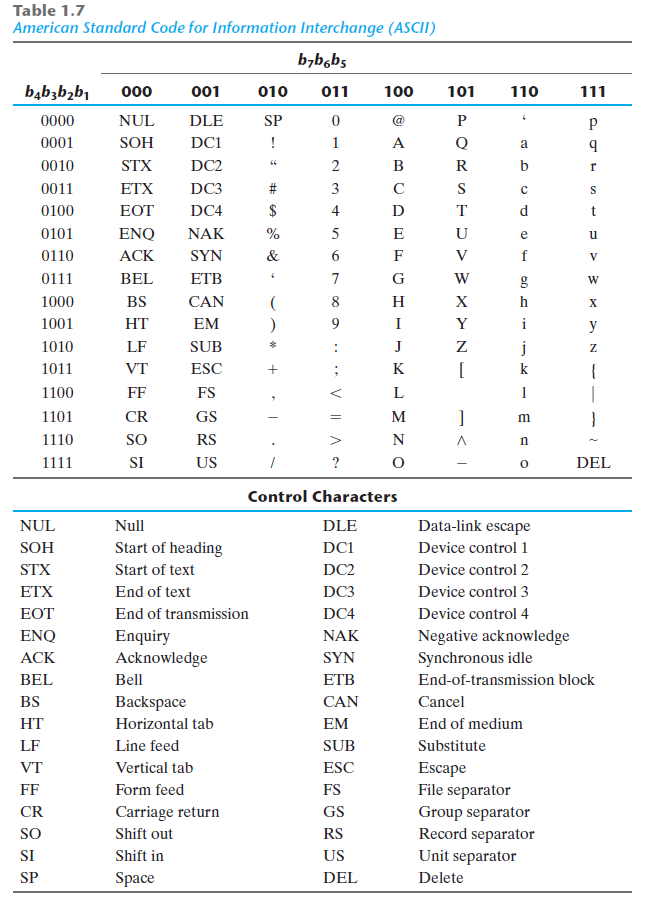
\includegraphics[width=0.8\linewidth]{1.png}
    \caption{ASCII CODE}
    \label{fig:enter-label}
\end{figure}
\subsection{Error Handling Code}
To detect errors in data communication, an additional parity bit is added to ASCII characters, ensuring an even or odd number of 1’s. Even parity is commonly used. 

At the sender's end, parity bits are generated, and at the receiver's end, they are checked. If a parity error is detected, the receiver sends an NAK (Negative Acknowledge) signal:

\[
\text{NAK} = 10010101
\]

This prompts retransmission. If no error is found, an ACK (Acknowledge) signal is sent:

\[
\text{ACK} = 00000110
\]

If repeated errors occur, manual intervention is required.
\end{document}
